
\section{Primeira Questão (6 pts)}

\subsection{Análise Analítica}

\numberwithin{equation}{section}
\numberwithin{figure}{section}

Um fluido de viscosidade $\mu$ e massa específica $\rho$ está em repouso
sobre uma placa horizontal quando ela começa a se mover com velocidade constante
$U_0$. A Figura \ref*{fig:geometriaQ1} exibe a geometria do problema.


\begin{figure}[h!]
    \caption{Geometria da questão 1.}
    \label{fig:geometriaQ1}
    \centering
    \centerline{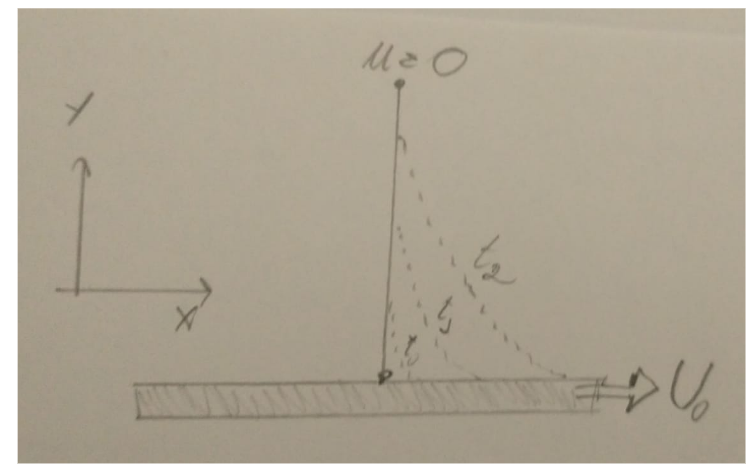
\includegraphics[scale=0.5]{geometriaQ1.png}}
    \par{Fonte: elaboração própria.}
\end{figure}

Como mostra a Figura \ref*{fig:geometriaQ1}, a linha média do fluido começa
a ser arrastada pelo movimento da placa, e a cada instante de tempo $t_0$,
$t_1$ e $t_2$ o movimento da placa atinge pontos cada vez mais altos
da linha média do fluido. Nesse cenário, a velocidade horizontal $u$ do
fluido é uma função de duas variáveis: posição vertical $y$ e tempo $t$.

A equação diferencial que modela o problema é

\begin{equation}\label{eq:modeloQ1}
    \diffp{u}{t} = \frac{\mu}{\rho} \diffp[2]{u}{y}
\end{equation}

\noindent com as seguintes condições de contorno:

\begin{equation}\label{eq:modeloQ1Contorno}
    \begin{cases}
        u(0, t) = U_0, & \textrm{Condição de contorno 1} \\
        u(H, t) = 0,   & \textrm{Condição de contorno 2} \\
        u(y, 0) =  0,  & \textrm{Condição inicial}       \\
    \end{cases}
\end{equation}

Veja que o problema é modelado por uma equação diferencial de segunda ordem 
em regime transiente, logo precisamos de duas condições de contorno e uma condição 
inicial.

No nosso sistema de coordenadas, $y = 0$ corresponde ao ponto do fluido
em contato com a placa, e $y = H$ é a altura máxima que iremos considerar na análise.
Note que, para $H$ suficiente grande, faz sentido assumir que o movimento da placa
não atinge esses pontos do fluido a uma grande distância da placa, de modo que
$u(H, t) = 0$.

O problema dado por \eqref{eq:modeloQ1} e \eqref{eq:modeloQ1Contorno} possui solução analítica dada por

\begin{equation}\label{eq:solAnaliticaQ1}
    u(y,t) = U_0 \left[1 - erf\left(\frac{y}{2\sqrt{\frac{\mu}{\rho}t}}\right)\right]
\end{equation}

\noindent em que $erf$ é a função erro dada por

\begin{equation}\label{eq:erf}
    erf(\beta) = \frac{2}{\sqrt{\pi}} \int_0^\beta e^{-x^2} \, dx
\end{equation}

Usando linguagem R e a IDE RStudio,
é possível obter a distribuição de velocidades do fluido
a partir da equação \eqref{eq:solAnaliticaQ1}, uma vez que a função erro $erf$
já está implementada em pacotes da linguagem. Usamos os seguintes parâmetros:

\begin{itemize}
    \item Domínio de análise vertical: $H=10 \un{cm}$
    \item Domínio de análise no tempo: $T=1 \un{s}$
    \item Viscosidade: $\mu=0.29 \un{ kg m$^{-1}$ s$^{-1}$}$
    \item Massa específica: $\rho=891 \un{kg m$^{-3}$}$
    \item Velocidade da placa: $U_0 = 1 \un{m/s}$
\end{itemize}

A Figura \ref*{fig:velocidadesAnaliticaQ1}
exibe os valores de $u(y,t)$ em função do tempo e posição vertical obtidos através da equação
\eqref{eq:solAnaliticaQ1} com os parâmetros acima.

\begin{figure}[h!]
    \caption{Velocidade $u$ do fluido função da posição e tempo.}
    \label{fig:velocidadesAnaliticaQ1}
    \centering
    \centerline{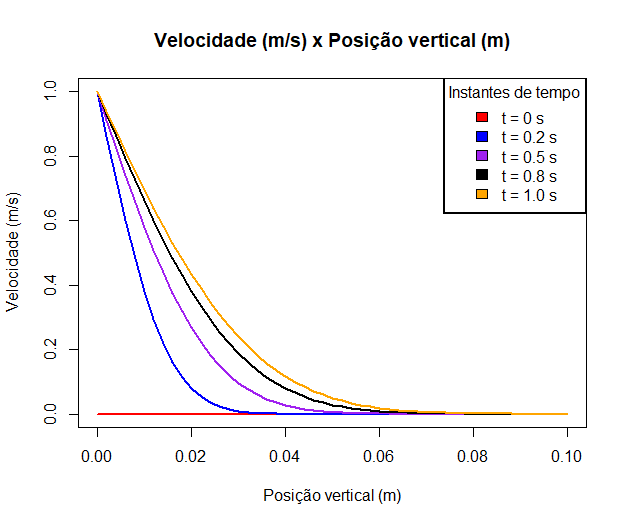
\includegraphics[scale=0.5]{velocidadesAnaltico.png}}
    \par{Fonte: elaboração própria.}
\end{figure}

As velocidades obtidas analiticamente na Figura \ref*{fig:velocidadesAnaliticaQ1} são condizentes
com o analisado da geometria na Figura \ref*{fig:geometriaQ1}. Conforme o tempo passa,
os pontos do fluido apresentam velocidade $u$ cada vez maior, uma vez que são arrastados
pelo movimento da placa. Os pontos em $y > 7 \un{cm}$ já não sofrem nenhum efeito
do movimento da placa até $t = 1 \un{s}$.

Analisando os pontos específicos pedidos no exercício, temos

\[ u(3 \un{cm}, 0.5 \un{s}) = 0.096 \un{m/s} \]
\[ u(3 \un{cm}, 1 \un{s}) = 0.24 \un{m/s} \]

\subsection{Análise Numérica}

Uma vez entendido o que está acontecendo analiticamente, podemos fazer uma análise
numérica do problema usando o método de diferenças finitas. O primeiro passo
é discretizar a equação diferencial \eqref{eq:modeloQ1}, trocando os diferenciais
por diferenças.

\begin{equation}\label{eq:modeloQ1Discretizado}
    \frac{u^{p+1} - u^p}{\Delta t} = \frac{\mu}{\rho} \frac{u_{i+1} - 2u_i + u_{i-1}}{\left(\Delta y\right)^2}
\end{equation}

Em \eqref{eq:modeloQ1Discretizado} adotamos a seguinte simbologia:

\begin{itemize}
    \item Sobrescrito $p$: indica o tempo da velocidade $u$. $p$ indica o tempo atual, $p + 1$ o próximo tempo
    \item Subscrito $i$: indica a posição vertical da velocidade $u$. $i$ indica a posição atual, $i + 1$ a próxima posição
    \item $\Delta t$: intervalo de discretização no tempo
    \item $\Delta y$: intervalo de discretização no espaço (vertical)
\end{itemize}

Assim, a linha média da Figura \ref*{fig:geometriaQ1} é discretizada em $H / \Delta y$ elementos de
comprimento $ \Delta y$, e o tempo é transcorrido a partir de $t = 0$ até $t = T$ em intervalos de  
$ \Delta t$. Vamos reescrever \eqref{eq:modeloQ1Discretizado} de modo a expressar a 
velocidade futura em função da velocidade antiga. 








